%!TEX root = ../docu.tex
\section{Projektplanung}
\label{proj}
\subsection{Arbeitspakete und Planung}
Bei der arbeit im team stellt sich häufig die frage wie programmfeatures bugs und allgemeine änderungen am quellcode durchgeführt werden bzw von welcher person.

hierführ gibt es viele vorgehenweisen. eine der höufigsten sit das anfertigen von sogenannten arbeitspaketen. diese beinhalten das vorher definierte ziel und jene schritte die zur erreichung des ziel nötig sind und welche anforderungen das ziel erfüllen muss.

ein solches arbeitspaket wird anschließend bewertet ud im aufwand eingeschätzt. das so erstellte arbeitspaket kann jetzt einem bearbeiter zugeteilt werden.

abhängigkeiten von arbeitspaketeten oder solche die auf einander aufbauen spielen eine gesonderte rolle. schnittstellen zwichen verschiedene in den paketen implentierte programmkomponenten müssen genau definiert werden umd spätere fehler oder inkompatibilität auszuschließen.

Die verwaltung de rpakete und zuweisung variiert je nach teamgröße. weit verbreitet sind Trac\footnote{http://trac.edgewall.org/}, Bugzialla\footnote{http://www.bugzilla.org/} sowie Redmine\footnote{http://www.redmine.org/}. Für ein Team mit kleinerer anzahl von mitgliedern empfehlen sich solche systeme nicht.

die wartung und konfiguration ist zu aufwendig die zeitkosten und nutzen stehen in keinem vertretbaren verhältnis.

für die umsetzung des projektes wurde daher auf ein managemnttool names Trello\footnote{https://trello.com/} verwendet. es realisiert eine managemnt mehtode namens \textit{Kanban} welche von Auomobielhersteller Toyota entwickelt wurde.

\subsubsection{Kanban}

die funktionsweise von kanban kann auf ein paar wesendliche bestandweile deferenziert werden. zunächst werden stadien definiert. jeh nach projektumgebung varrieren diese stadien. für die entwicklung von anwendungen sind folgende stadien aussreichen. zu beginn ist ein paket im stadium nicht zugewiesen bzw neu. das nächste stadium ist das stadium zugewiesen gefolgt vom stadium in bearbeitung. anshcließend wandert das areitspaket in das stadium test und von dort aus in das stadium beendet.

das system ist sehr üersichtlich da alle pakete auf einen blick ersichtlich sind sowie welche person für das jeweilige arbeitspaket zuständig ist.\newpage

deweiteren kann man sofort erkkenen in welchen stadium sich gerade welches paket befindet. das gnaze system ist daher sehr überischtlich und einfach strakturiert.

de vorteile von kanban liegt an der hoehen transparenz der aller abreitspakete und deren gegenwertigen status. die einführung und umsetzung sind resourcenschonend und schnell. der umgang mit kanban ist elicht zu erlenen und gerade für kleienr teams zu empfehlen.

\begin{figure}
\begin{center}
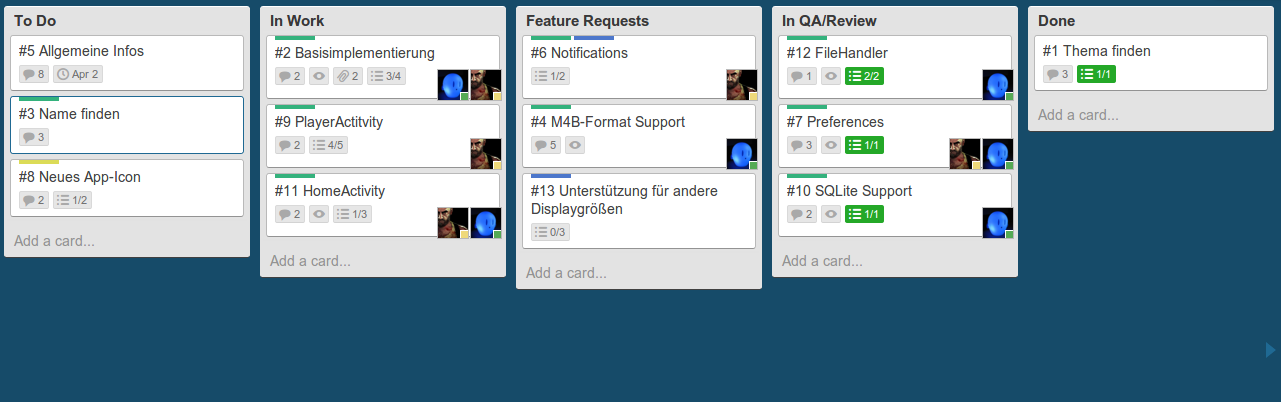
\includegraphics[scale=0.35]{images/kanban}
\caption{Kanbanboard mit verschiedneen arbeitspacketen}
\label{kanban}
\end{center}
\end{figure}

in der abbildung \ref{kanban} ist ein kanban.board abgebildet. sie durchlaufen verschiedene stadiun und wandern von der linken zu rechten seite des boards.

abgeshclossene packete werden nach einiger zeit vom brett genommen um die übersichlichkeit zu erleichtenr. solche baord können in papiervor oder auch auf eletronischen wege simuliert werden. eine elektronische variante wie sie im abgearbeiteten projekt verwendet wurde , wurde genanntan. weitere einzelheiten könn aus der literaturquelle \cite{9783898647304} entnommen werden.

\subsection{Entwicklungsumgebung}
für das arbeiten mit der umfangreichen Android Api empfielt es sich snadart entwickerwerkzeuge wie Eclipse zu wendenden. dies gewährleistet einen schnellen umgang mit allen bestnadweilen der Android SDK.

Desweitern können die loggaten schnell ausgewertet werden und fehler identifiziert werden. desweiteren können ähnluch wie bei der Programmierung von Java Anwendungen test verfasst werden und ein debuging erfolgen.

Eclips bietet eine autoverfvollständigung und eine typprüfung vor der kompilierungdes codes. Eclipse ist weiterhin in der lage viele codeabschnitte automatishc zu erzeugen und somit entwicklungsschritte zu beleunigen.

wichtig bei der arbeit mit einer ide wie eclipse ist die integratin dessdks um die für die entwicklung von android applikationen bereitgestellten werkzeuge nutzen zu können. heirzu gehören verschiedene debugging sowie kompilerwerkzeuge die die entwicklung erleichtern und hilfestellung leisten sollen.

\subsection{Versionsverwaltung des Quellcode}
Die versionierung von quellcode spielt eine große rolle bei der entwicklung von software. hierbei werden änderungen am quellcode zeitlich erfasst um einen chonologischen verlauf von änderungen festzuhalten und die aktualität des codes zu gewährleisten.

für diesen zweck gibt es verschiedene lösungsmöglichkeiten. weit verbreitet sind die versionierungssysteme SVN und GIT.
SVN ist ein zetralles versionierungssystem für dateien.  es gibt eine zentrale versionierungsstelle zudem sich klienten verbinden könen und ädnerungen einreichen können.

die wahl für die versionskontrolle viel auf GIT. GIT verfolgt eine andere stretegie. änderungen werden dezentral verwaltet. im folgenden sollen die wesentlichen aspekte von GIT genannt werden.

\textbf{kein zentraler server}

jeder benutzer hat eine exakte kopie der versionierung und ihren verlauf. alle arbeiten können daherer größtenteils ohne netzwerkzugriff ausgeführt werden.

\textbf{Datenaustausch}

der austausch von daten kann über viele protokolle und arten abgewickelt werden. der austaushc ist sehr felexibel und sicher, wenn für die übertragung geeignete abgesicherte protokolle verwendet werden.


\textbf{Kryptographische Sicherheit der Projektgeschichte}

Wären der des versionierungsprozesses wird ein eindeutiger Hash erzeugt welches den gesamten verlauf zur aktuellenv ersion wiederspiegelt eine anchträgliche änderung ist somit nciht möglick bzw kann nicht verschleiert werden. Gelöschte informationen bleiben erhalten und können weiderhergestellt werden.

Durch die dezentralisierung der versionierung muss dennoch ein austausch der daten zwichen den teammitgliedern gewährleistet sein.

hierfür gibt es verschiedene möglichkeiten unter anderem eine gemeinsame austauschstelle. diese austaushcstellen fungieren als vermitltungs udn samelpuntken. es besteht die möglichkeit solch einen punkt selber zu betreiben oder kostenlose anbieter wie GitHub\footnote{https://github.com/} zu verwenden.

